\documentclass{standalone}
\usepackage[utf8]{inputenc}
\usepackage{newtxtext}
\usepackage{newtxmath}
\usepackage[italic]{hepnicenames}
\makeatletter\def\@shiftlen@anti@gen@bar{0mu}\makeatother
\usepackage[svgnames]{xcolor}
\usepackage{tikz-feynhand}


\begin{document}
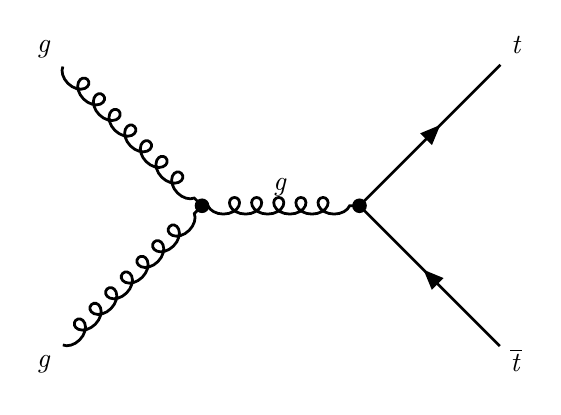
\begin{tikzpicture}
  \setlength{\feynhandlinesize}{1.0pt}
  \tikzfeynhandset{every dot={/tikz/color=Black},}
  \begin{feynhand}
    \vertex [particle, Black] (g1) at (-3.0, 2.0) {\Pg};
    \vertex [particle, Black] (g2) at (-3.0, -2.0) {\Pg};
    \vertex [particle, Black] (t1) at (3.0, 2.0) {\Pqt};
    \vertex [particle, Black] (t2) at (3.0, -2.0) {\Paqt};
    \vertex [dot, Black] (gg) at (-1.0, 0.0) {};
    \vertex [dot, Black] (gt) at (1.0, 0.0) {};
    \propagator [gluon, Black] (g1) to (gg);
    \propagator [gluon, Black] (g2) to (gg);
    \propagator [gluon, Black] (gg) to [edge label=\Pg, color=Black] (gt);
    \propagator [fermion, Black] (gt) to (t1);
    \propagator [fermion, Black] (t2) to (gt);
  \end{feynhand}
\end{tikzpicture}
\end{document}
